\documentclass{llncs}
\usepackage{color}
\usepackage{soul}
\usepackage{cite}
\usepackage{array}
\usepackage{listings}
\usepackage{graphicx}

\usepackage{url}
\newcommand{\starpar}[1]{\par{\footnotesize $\star$ \hl{#1}\par}}

\lstset{basicstyle=\scriptsize,breaklines=true,breakindent=60pt,xleftmargin=20pt,numberstyle=\tiny,numbersep=5pt,language=C}

\begin{document}

\title{Recovering OpenSSL ECDSA Nonces Using the \textsc{Flush+Reload} Cache Side-channel Attack}

\maketitle

\begin{abstract}
\end{abstract}

\section{Introduction}

\starpar{Contributions:}
\starpar{Demonstrate that the \textsc{Flush+Reload} attack is generic}
\starpar{Show a weakness in the Montgomery Ladder implementation of group multiplication}
\starpar{Show that even minor branch dependence on secret data is vulnerable}
\starpar{Analysis of partial nonce exposure?}
\section{Preliminaries}
\subsection{ECDSA}
\subsection{The Montgomery Ladder}
\subsection{The \textsc{Flush+Reload} attack}
\section{Attacking OpenSSL ECDSA}
OpenSSL is one of the most common open-source cryptographic libraries.
It provides a set of cryptographic services, including public and shared key encryption 
algorithms and public key signature algorithms.

OpenSSL's implementation of ECDSA uses the Montgomery ladder algorithm for scalar multiplication
on the Elliptic Curve.
We use this implementation to demonstrate that na{\"\i}ve implementations of the Montgomery ladder are
susceptible to the \textsc{Flush+Reload} attack.

Listing~\ref{lst:openssl} shows the relevant section of the implementation of the Montgomery ladder in OpenSSL version 1.0.1e.
The bits of the multiplication scalar are stored in the word array \texttt{scalar->d}.
The outer loop, at lines~268 to~286 traverses over the words representing the scalar.
The inner loop, at lines~271 to~284 traverses the bits in each word.
Line~273 tests the bit. 
For each bit the implementation executes a group add followed by a group double.
If the bit is set, the implementation uses lines~275 and~276.
For clear bits it uses lines~280 and~281.

\begin{lstlisting}[numbers=left,firstnumber=268,float=htb,caption=OpenSSL Implementation of the Montgomery Ladder,label=lst:openssl]
for (; i >= 0; i--)
{
    word = scalar->d[i];
    while (mask)
    {
        if (word & mask)
        {
            if (!gf2m_Madd(group, &point->X, x1, z1, x2, z2, ctx)) goto err;
            if (!gf2m_Mdouble(group, x2, z2, ctx)) goto err;
        }
        else
        {
            if (!gf2m_Madd(group, &point->X, x2, z2, x1, z1, ctx)) goto err;
            if (!gf2m_Mdouble(group, x1, z1, ctx)) goto err;
        }
        mask >>= 1;
    }
    mask = BN_TBIT;
}
\end{lstlisting}

As the listing demonstrates, the Implementation is very regular.
For each bit, the implementation executes exactly the same sequence of operations.
The only differences between set and clear bit are the lines that invoke these operations.
Our attack exploits this difference.
The attack probes the cache lines used by OpenSSL to identify the branch taken by the \texttt{if}
statement in line~273.
From this information we can deduce the value of the bit and by repeating the attack throughout
the execution of the scalar multiplication we can recover most of the bits of the nonce.


The mapping of source lines to cache lines in our build of OpenSSL is depicted in Diagram~\ref{dgm:memory}.
The machine code created from source lines~273 to~282 covers the virtual memory address range 0x0812130C
to 0x081213e8.
This range spans four cache lines, marked $A$, $B$, $C$ and $D$.
The attacks observes the sequence of cache access made by the processor when executing the code.


\begin{figure}[htb]
\centering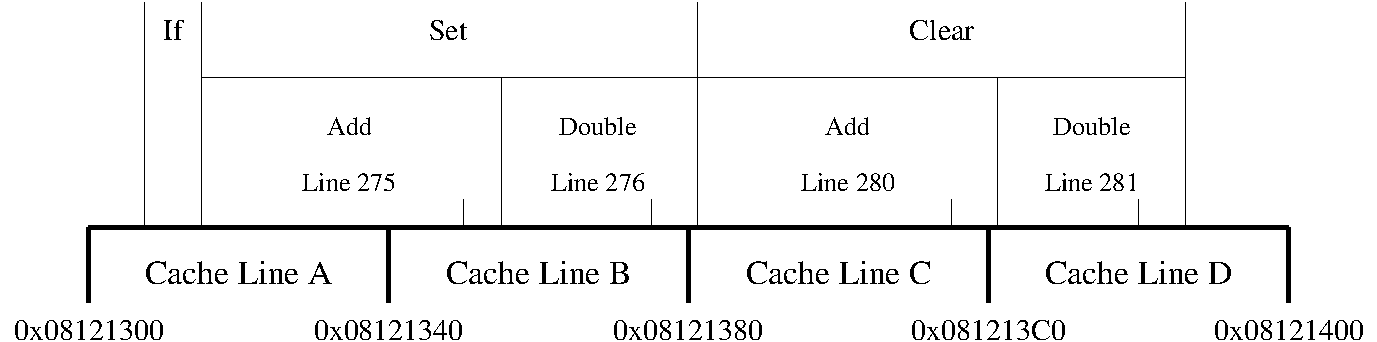
\includegraphics[width=\columnwidth]{images/memory}
\caption{Mapping from Source Code to Memory\label{dgm:memory}}
\end{figure}


\starpar{required, actual and observed cache access sequences}

The \texttt{if} statement at line~273 is executed for each bit.  
The code of this statement is in cache line $A$, hence this line is accessed when processing of a bit starts.
For set bit, the processing continues with source line~275, which maps to cache lines~$A$ and~$B$.
The actual call to the group add function occurs at address 0x08121347.
(See mark in Diagram~\ref{dgm:memory}.)
After a delay for computing the group add, execution continues in cache line~$B$ to process the return value and 
to invoke the group doubling function.
The group doubling function returns to cache line~$B$ and execution leaves the \texttt{if} body at cache line~$D$.

Hence, the sequence of cache line accesses required for a set bit is: $A$, $B$, \textit{add}, $B$, \textit{double}, $B$, $D$.
Similarly, for a clear bit, the sequence is: $A$, $C$, \textit{add}, $C$, $D$, \textit{double}, $D$.

Processor optimisations may add otherwise unrequired cache line accesses.
The spatial prefetching optimisation~\cite{intel12optimization} pairs adjacent cache lines and tries to bring both cache lines
when there is a miss on one of the pair's line.
For example, when there is a cache miss on cache line~$A$, the spatial prefetcher may attempt to prefetch cache line~$B$
and vice versa.

Another optimisation that can cause additional cache line access is speculative execution~\cite{uht95disjoint}.
With speculative execution, the processor follows both \hl{arms} of a conditional branch before evaluating
the condition.
When the condition is evaluated, the processor commits to the pre-processed computation of the correct \hl{arm},
disposing of the computation done for the other \hl{arm}. 
In the case of OpenSSL this means that even before evaluating the bit, 
the processor may start processing both line~275 and line~280, triggering memory loads from cache lines~$A$, $B$ and $C$.




\section{Results}
\section{Discussion}
\section{Related Work}
\section{Conclusions}

\bibliographystyle{splncs}
\bibliography{Euro2014}

\end{document}

